\documentclass[tikz,border=6pt]{standalone}
\usetikzlibrary{arrows.meta,calc,decorations.pathreplacing,positioning,fit,shapes.callouts}
\definecolor{ksupurple}{HTML}{512888}
\definecolor{orange}{HTML}{CA7C1B}

\begin{document}
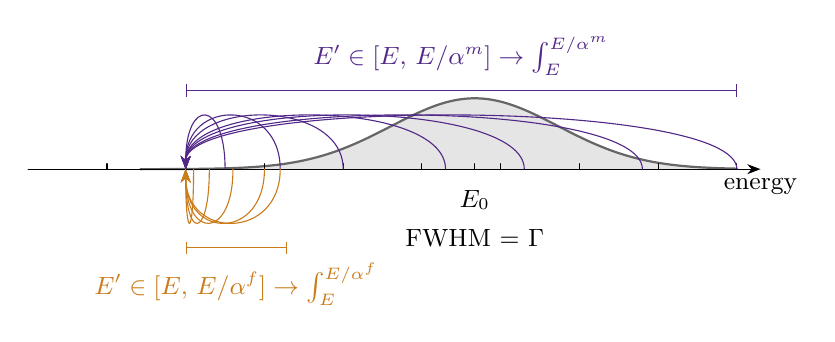
\begin{tikzpicture}[
  >=Stealth, line cap=round, line join=round,
  mod/.style  ={ksupurple,  thin},
  fuel/.style ={orange, thin},
  eqtxt/.style={font=\small},
  resband/.style={fill=black!10,draw=black!50},
  every node/.style={font=\small}
]

\def\Emin{1}          % axis min (arbitrary units)
\def\Emax{10}         % axis max
\def\Eo{3.0}          % target energy E
\def\am{0.30}         % alpha^m (moderator)
\def\af{0.70}         % alpha^f (fuel)
\pgfmathsetmacro{\EoOverAm}{\Eo/\am}
\pgfmathsetmacro{\EoOverAf}{\Eo/\af}

\pgfmathsetmacro{\Er}{6.67}       % resonance energy
\pgfmathsetmacro{\Gnarrow}{0.2} % narrow width
\pgfmathsetmacro{\Gwide}{2.50}   % wide width
 

\pgfmathsetmacro{\Emleft}{\am*\Er} % alpha^m * Er (left edge of moderator step)
\pgfmathsetmacro{\Efleft}{\af*\Er} % alpha^f * Er (left edge of fuel step)

% --- Resonance as a curve (Gaussian or SLBW) -------------------------
% Toggle one of these:
\def\drawGaussian{1}  % 1 = draw Gaussian
\def\drawSLBW{0}      % 1 = draw SLBW/Lorentzian (set the other to 0)

% Which width to use in this figure (use \Gnarrow or \Gwide)
\pgfmathsetmacro{\GammaUse}{\Gwide}

% Peak height for the curve (keep under the arc height 0.9 so it doesn't collide)
\pgfmathsetmacro{\Ares}{0.90}

% --- Gaussian: use FWHM Gamma -> sigma conversion: Gamma = 2 sqrt(2 ln 2) sigma
\pgfmathsetmacro{\sigma}{\GammaUse/(2*sqrt(2*ln(2)))}
\pgfmathsetmacro{\xminG}{max(\Emin,\Er-4*\sigma)}
\pgfmathsetmacro{\xmaxG}{min(\Emax,\Er+4*\sigma)}

% --- SLBW/Lorentzian “shape-only”: peak height A and FWHM Gamma
% y(x) = A * (0.25*Gamma^2) / ((x-Er)^2 + 0.25*Gamma^2)
\pgfmathsetmacro{\xminL}{max(\Emin,\Er-6*\GammaUse)}
\pgfmathsetmacro{\xmaxL}{min(\Emax,\Er+6*\GammaUse)}

% --- Draw Gaussian band (fill + outline)
\ifnum\drawGaussian=1
  % light fill under the curve
  \path[fill=black!10, draw=none]
    (\xminG,0) --
      plot[domain=\xminG:\xmaxG, samples=181]
        (\x, {\Ares*exp(-((\x-\Er)^2)/(2*\sigma*\sigma))})
    -- (\xmaxG,0) -- cycle;
  % curve outline
  \draw[black!60, line width=0.8pt]
      plot[domain=\xminG:\xmaxG, samples=181]
        (\x, {\Ares*exp(-((\x-\Er)^2)/(2*\sigma*\sigma))});
\fi

% --- Draw SLBW/Lorentzian band (fill + outline)
\ifnum\drawSLBW=1
  \path[fill=black!10, draw=none]
    (\xminL,0) --
      plot[domain=\xminL:\xmaxL, samples=220]
        (\x, {\Ares*(0.25*\GammaUse*\GammaUse)/((\x-\Er)*(\x-\Er)+0.25*\GammaUse*\GammaUse)})
    -- (\xmaxL,0) -- cycle;
  \draw[black!60, line width=0.8pt]
      plot[domain=\xminL:\xmaxL, samples=220]
        (\x, {\Ares*(0.25*\GammaUse*\GammaUse)/((\x-\Er)*(\x-\Er)+0.25*\GammaUse*\GammaUse)});
\fi

% Label (keeps your original placement idea)
\node[black, below=4pt] at (\Er, -0) {$E_0$};
\node[black, below=4pt] at (\Er, -0.5) {FWHM = $\Gamma$};


% 
% \path[resband] (\Er-\G/2,-0.35) rectangle (\Er+\G/2,0.9);
% \node[black, below=4pt] at (\Er+\G/2+0.05, -0.25) {resonance, $\Gamma$};


\draw[->] (\Emin,0) -- (\Emax+0.3,0) node[below] {energy};
\foreach \x in {2,...,10} \draw (\x,0) -- ++(0,0.07);
\draw (\Er,0) -- ++(0,0.07);

\draw[ksupurple, |-|]
  (\Eo,1) -- node[above=2pt, mod] {$E' \in [E,\,E/\alpha^{m}] \rightarrow \int^{E/\alpha^m}_E$} (\EoOverAm,1);
\draw[orange, |-|]
  (\Eo,-1) -- node[below=2pt, fuel] {$E' \in [E,\,E/\alpha^{f}]\rightarrow \int^{E/\alpha^f}_E$} (\EoOverAf,-1);

\foreach \Ep in {3.5,4.2,5.0,6.3,7.3, 8.8, 10}
  \draw[mod,->, thin] (\Ep,0) .. controls ($( \Ep, 0)+(0,0.9)$) and ($(\Eo,0)+(0,0.9)$) .. (\Eo,0);

\foreach \Ep in {3.10, 3.3, 3.6, 4.0, 4.2}
  \draw[fuel,->, thin] (\Ep,0) .. controls ($( \Ep, 0)+(0,-0.9)$) and ($(\Eo,0)+(0,-0.9)$) .. (\Eo,0);
 
 
\end{tikzpicture}
\end{document}
